%\begin{figure*}[t]
%		\begin{minipage}{0.32\linewidth}
%			\centering
%			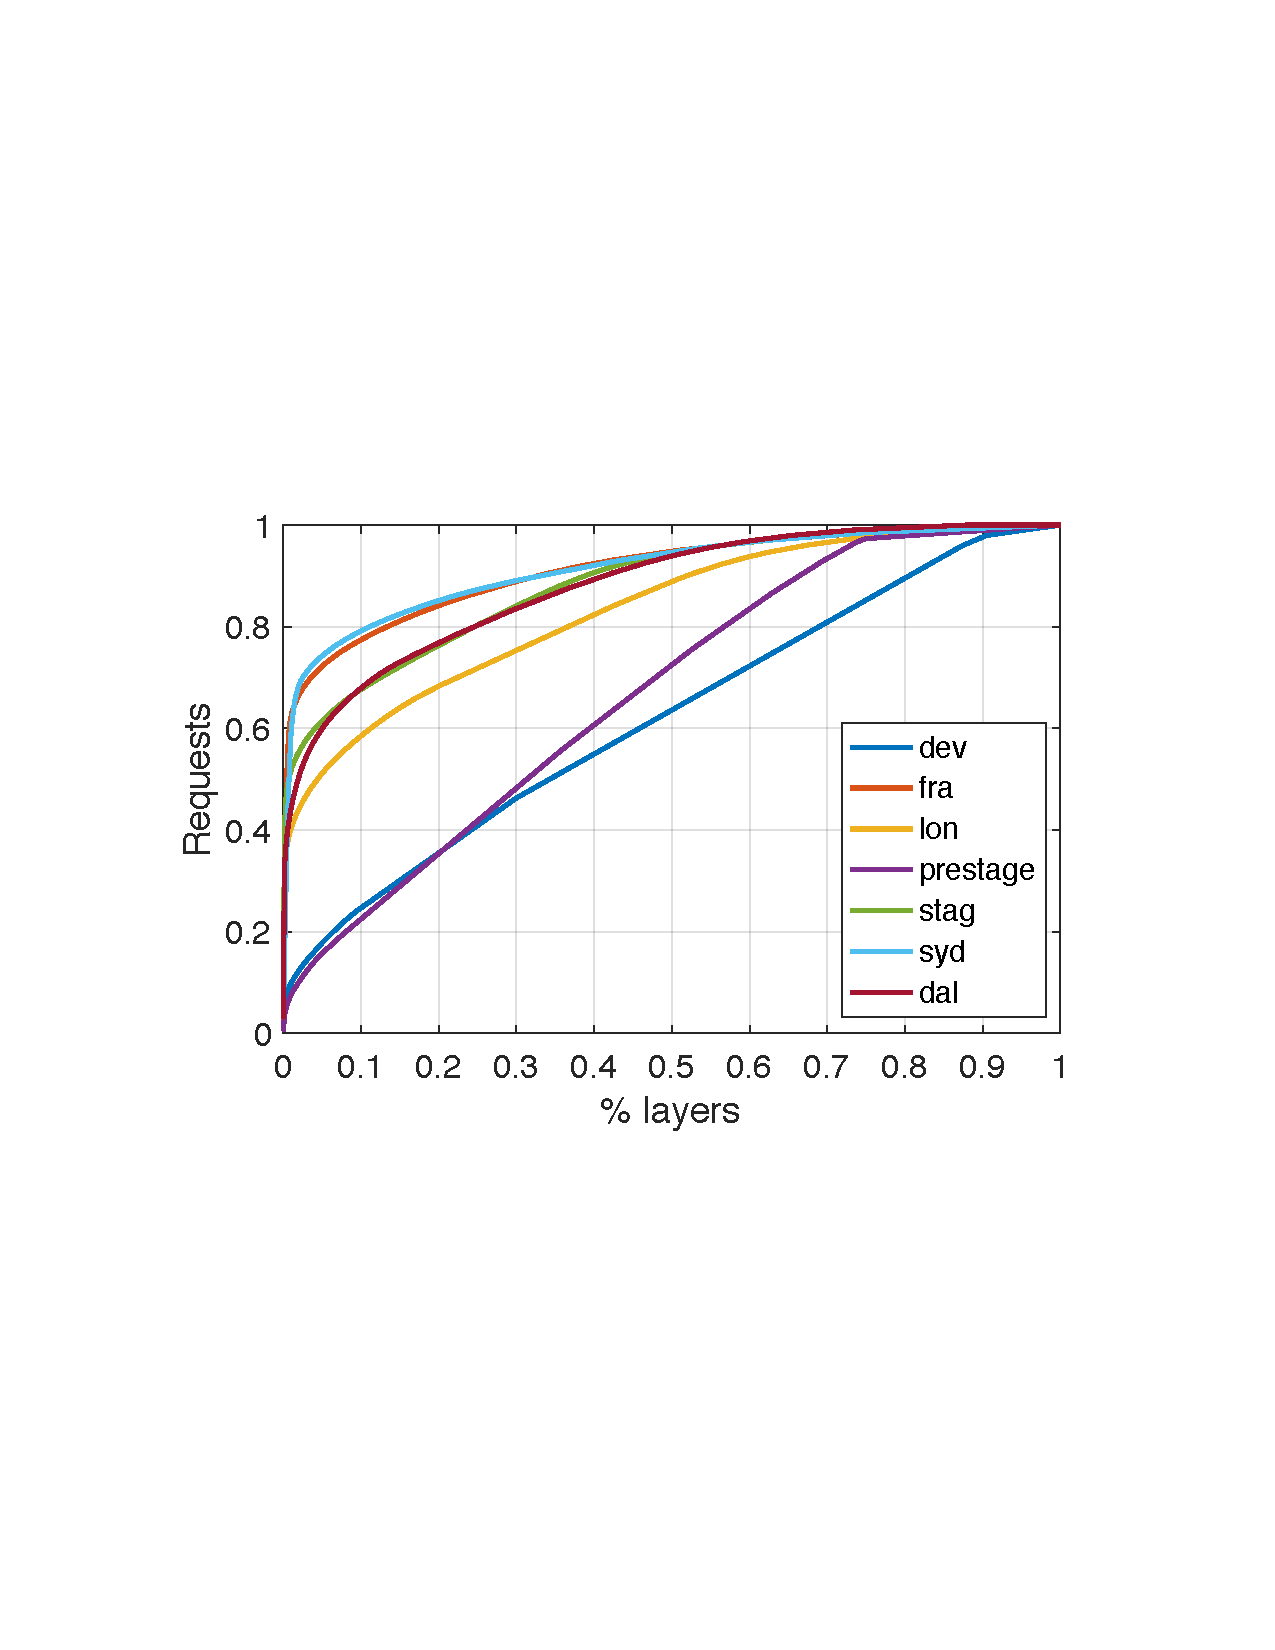
\includegraphics[width=1\textwidth]{graphs/layer_skewness.pdf}
%			%\caption{CDF of layer  count.}
%		%	\vspace{-3pt}
%			\label{fig:layer-skenwess}
%		\end{minipage}
%			\begin{minipage}{0.32\linewidth}
%				\centering
%				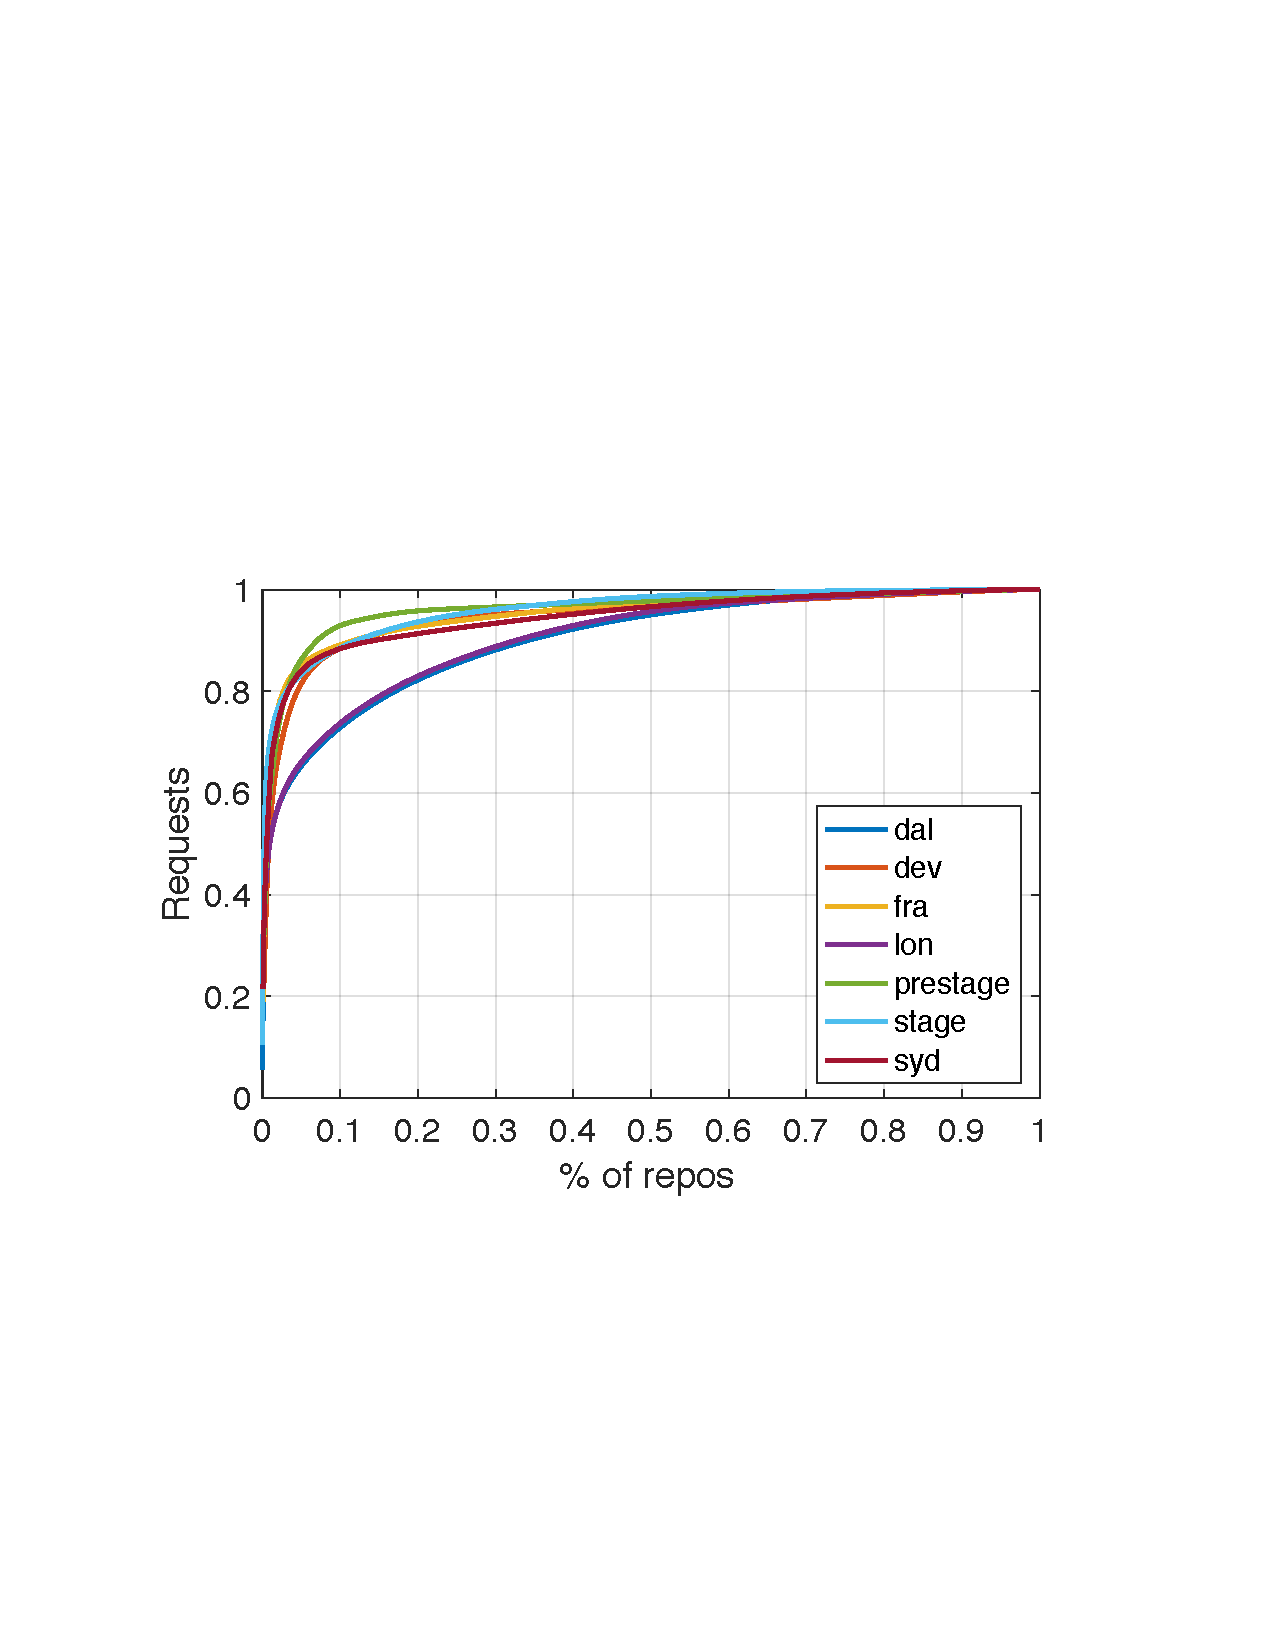
\includegraphics[width=1\textwidth]{graphs/repo-skewness.pdf}
%				%\caption{PDF of repository repulling probability.}
%				%	\vspace{-3pt}
%				\label{fig:repo-skewness}
%			\end{minipage}
%		\hfill
%		\begin{minipage}{0.32\linewidth}
%			\centering
%			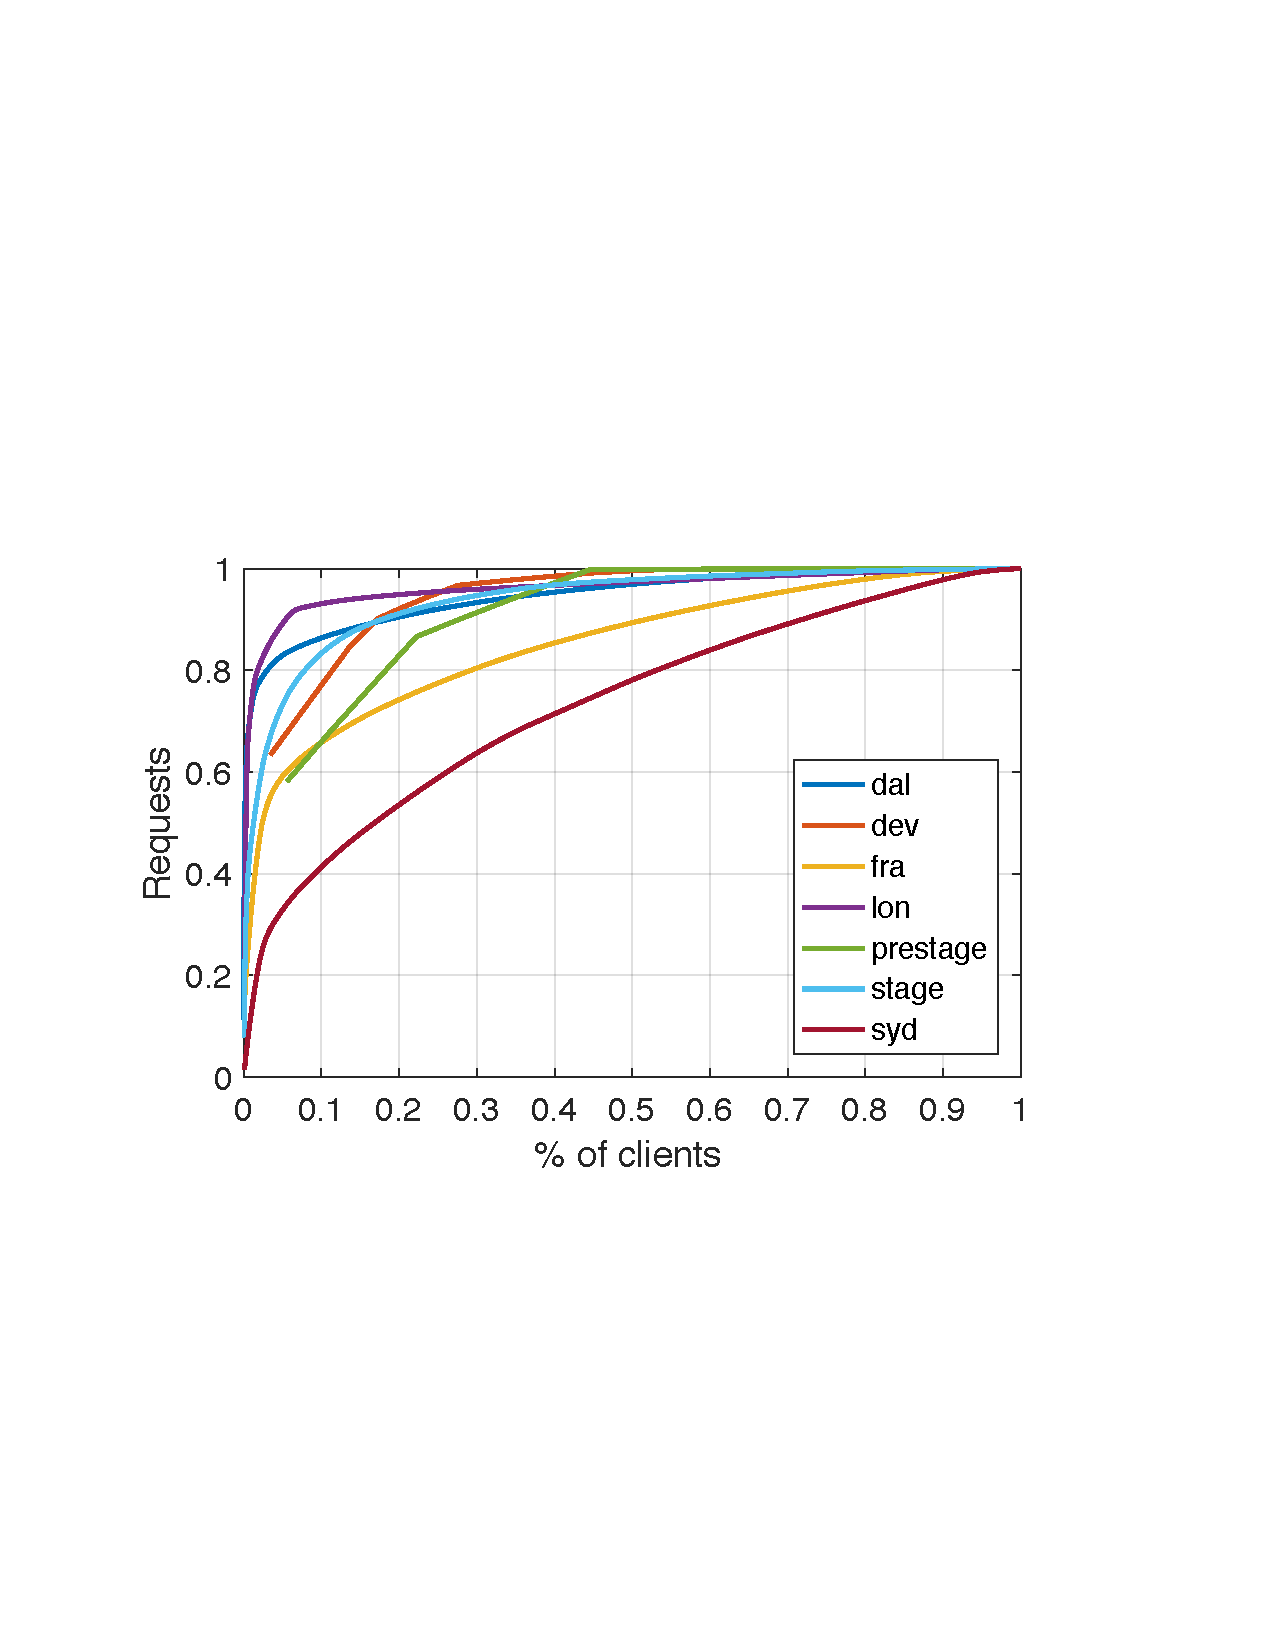
\includegraphics[width=1\textwidth]{graphs/client-skewness.pdf}
%			%\caption{PDF of client repulling probability.}
%			%	\vspace{-3pt}
%			\label{fig:client-skewness}
%			
%		\end{minipage}
%\caption{PDF of probability for layers, repositories, and clients.}
%%	\label{}
%\end{figure*}

\begin{figure*}[!t]
	\centering
	\subfigure[Layer repull count]{
		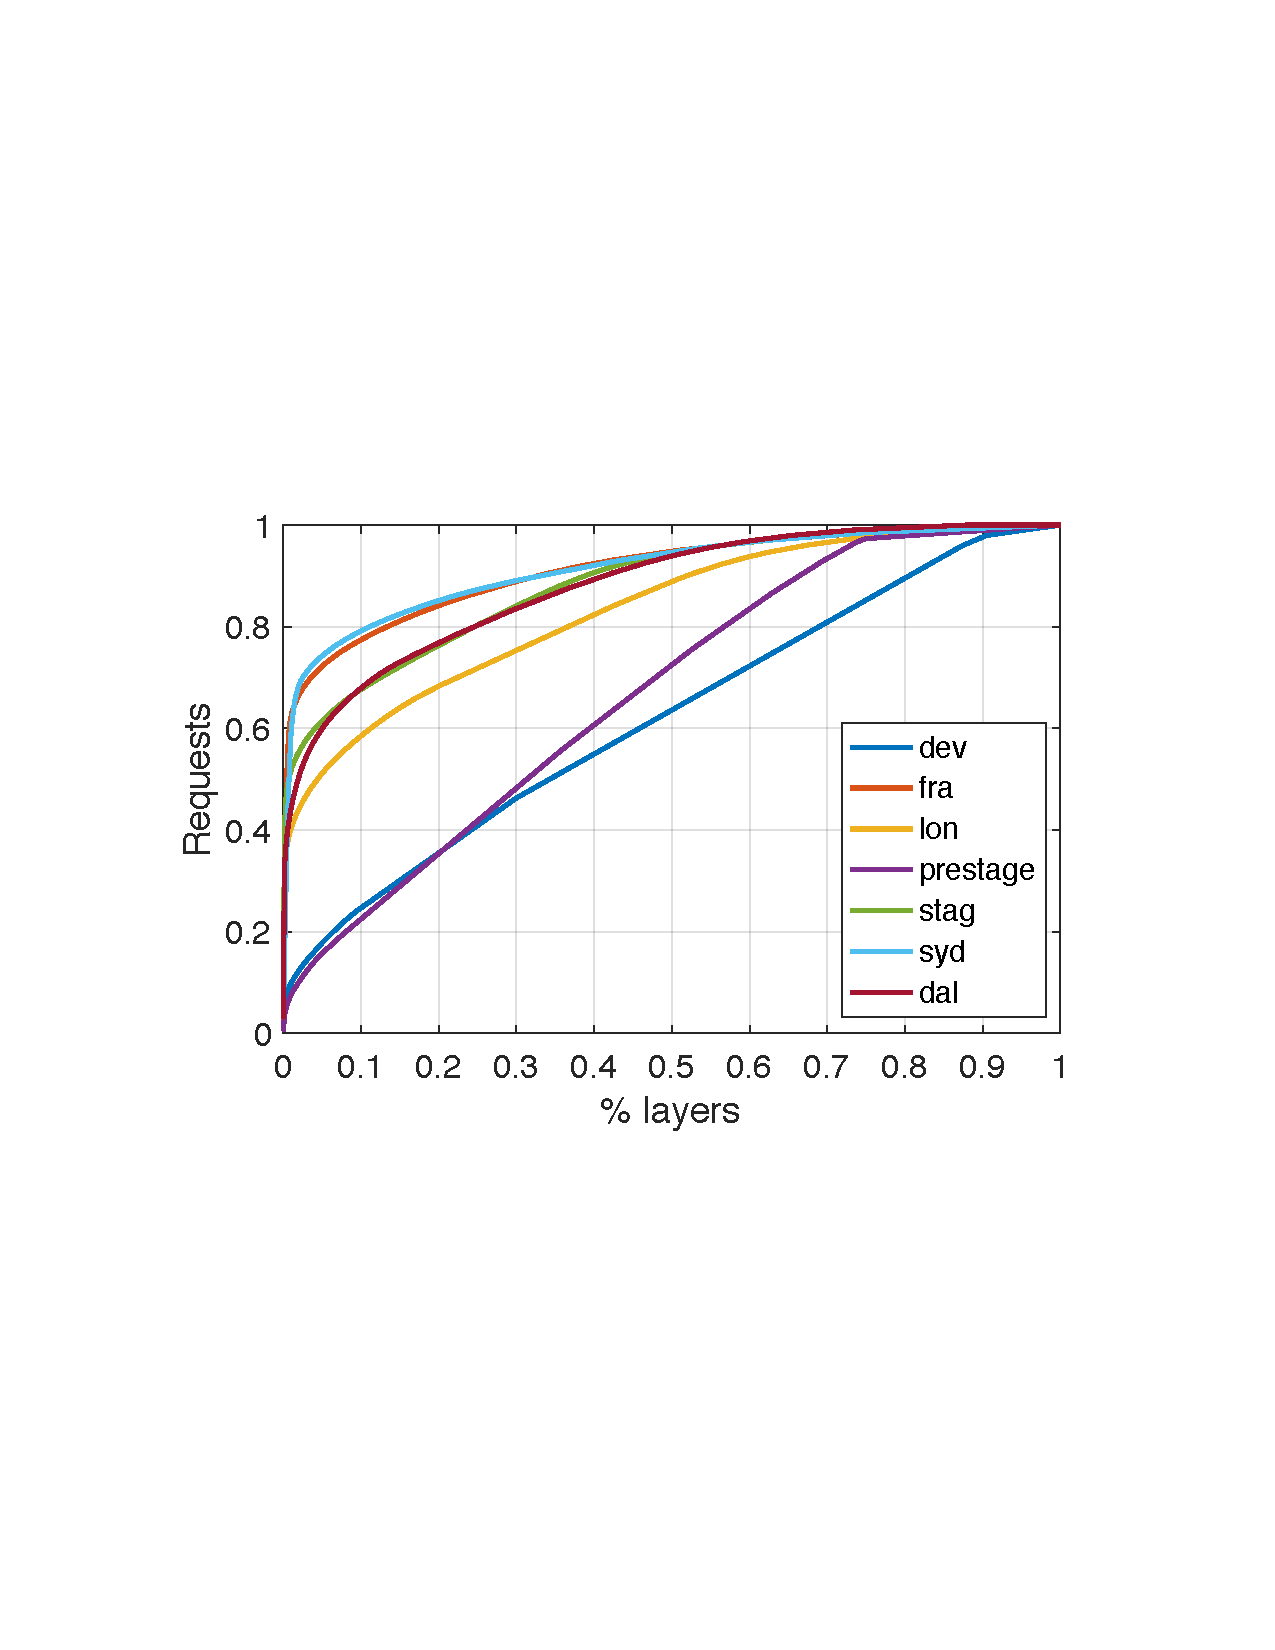
\includegraphics[width=0.2\linewidth]{graphs/layer_skewness.pdf}
		\label{fig:layer-skewness}
	}
	\subfigure[Repository repulling probability]{
		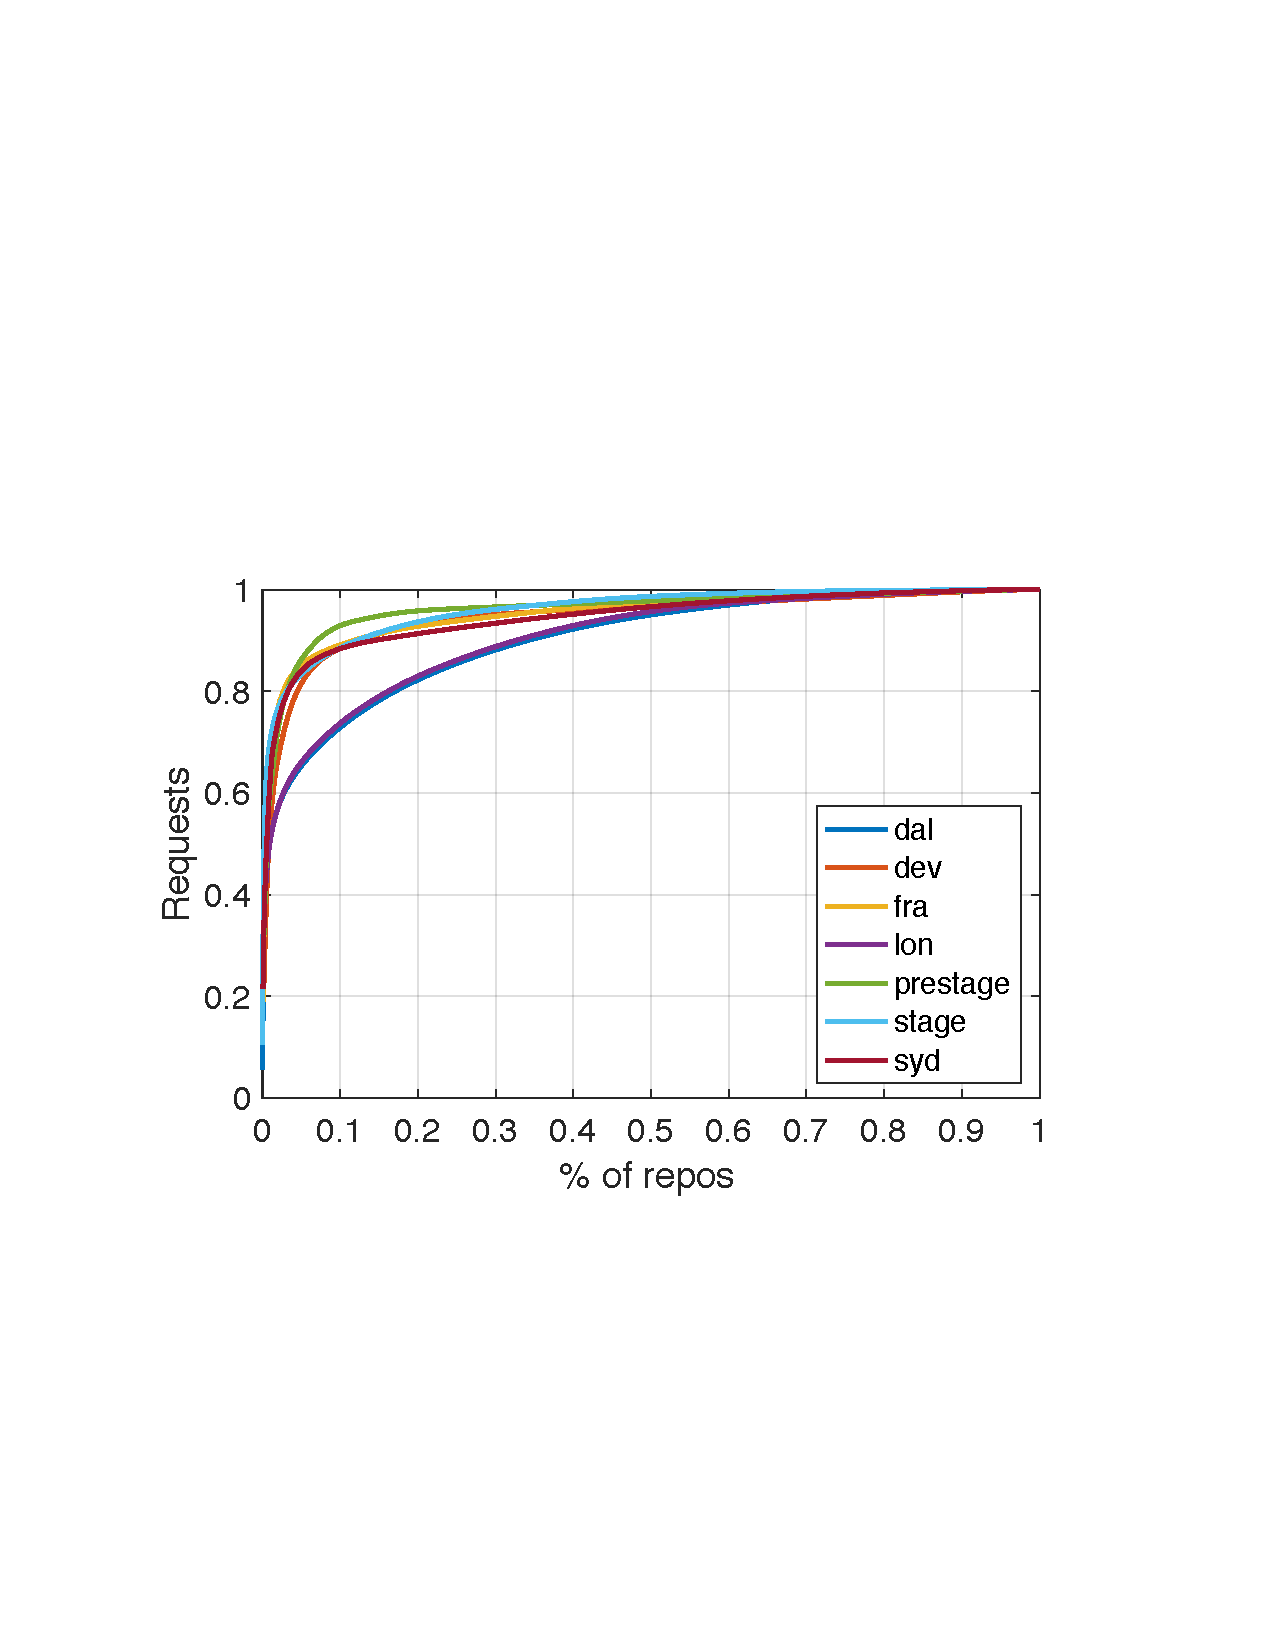
\includegraphics[width=0.2\linewidth]{graphs/repo-skewness.pdf}
		\label{fig:repo-skewness}
	}
	\subfigure[Client repulling probability]{
		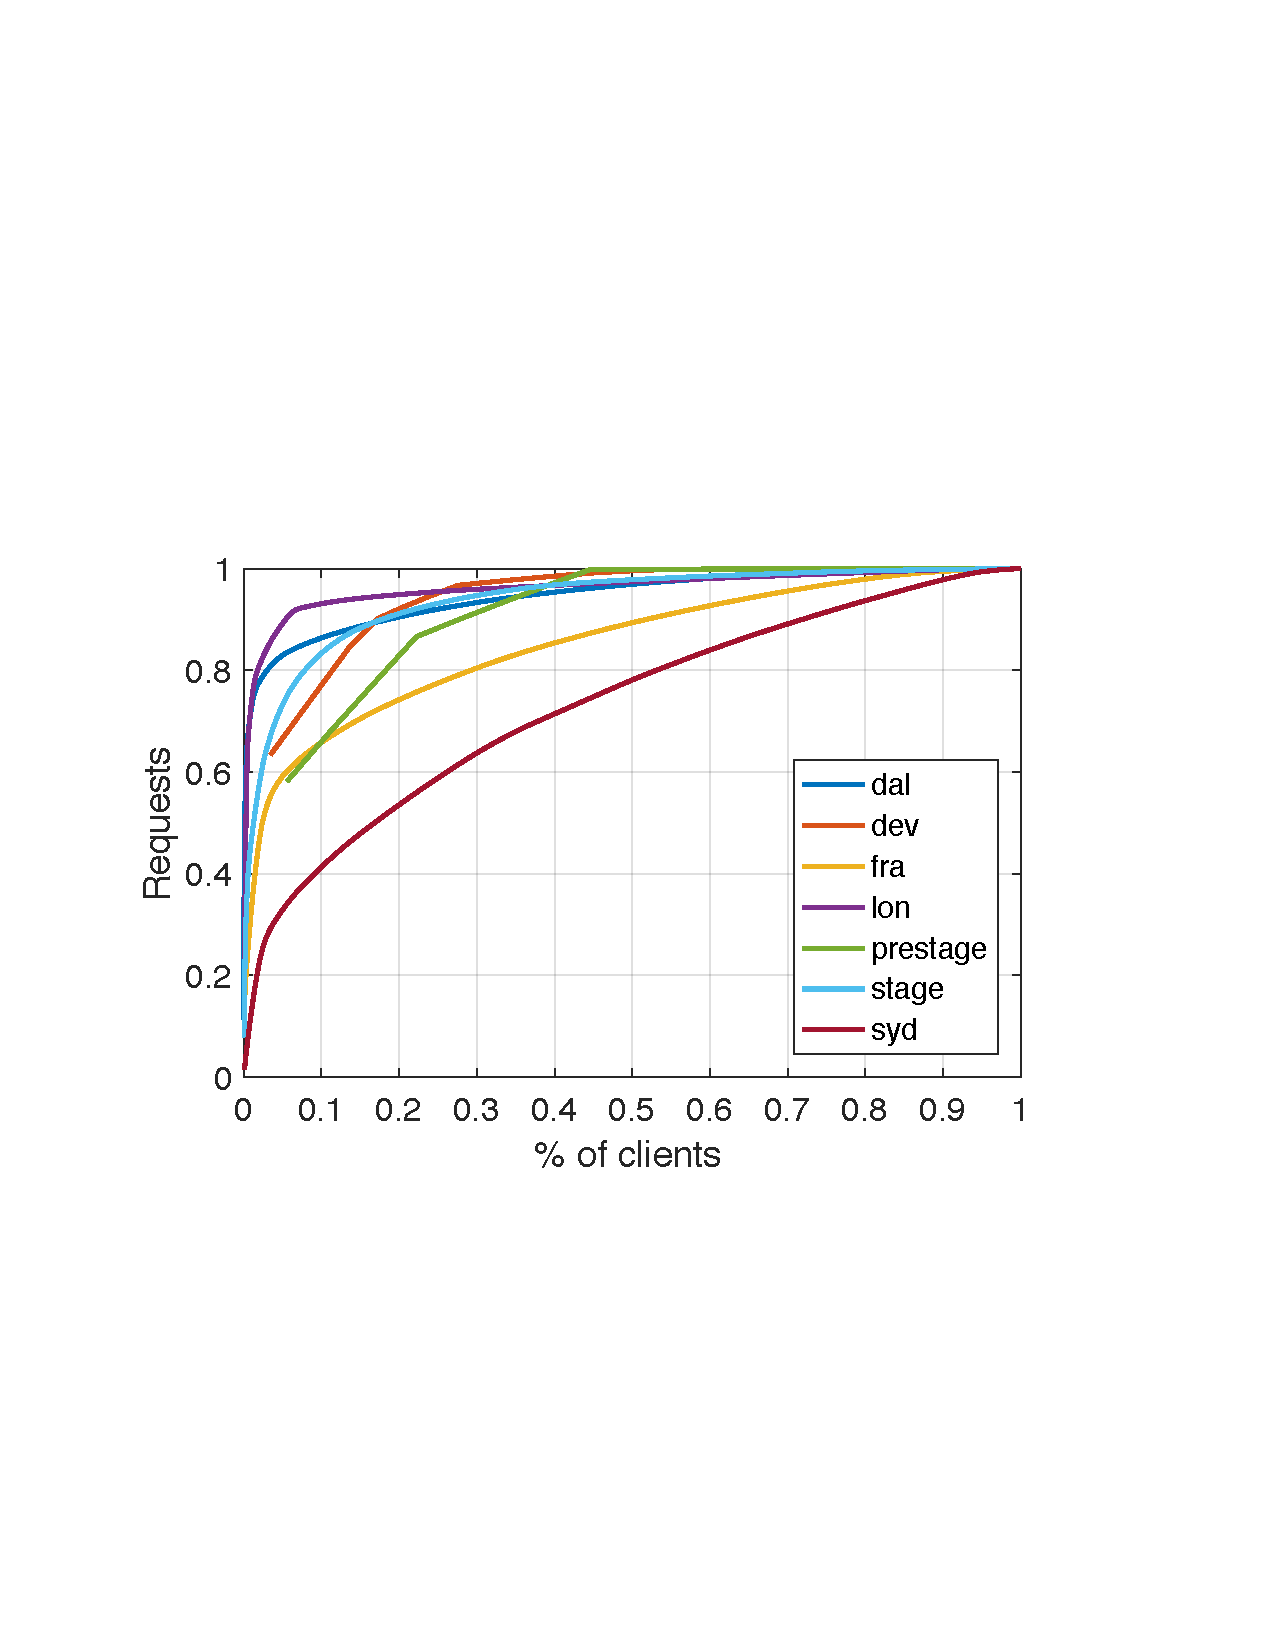
\includegraphics[width=0.2\linewidth]{graphs/client-skewness.pdf}
 	\label{fig:client-skewness}
	}
\caption{CDF of probability for layers, repositories, and clients.}
	\label{fig-skewness}
\end{figure*}